\section{背景}
近年,コンテンツをノード,コンテンツ間の関係性をエッジとみなしたグラフ表現・解析を行うことへの注目が高まっている.
Social Network Service の友人関係や,World Wide Web の参照関係などがグラフとして表現される代表例であり,年々これらの
グラフサイズは巨大化している.
\cite{ching2015one}では,2015 年時点で Facebook グラフのエッジ数は 1 兆を上回ると報告されており, 
今後もグラフサイズの巨大化は継続していくと予想される.
また,現在は単一主体によるグラフの集中管理が主流であり,コンテンツ間の関係性を定義するのはグラフの管理者である.
このような管理形態では,様々な主体が自由にコンテンツ間の関係性を見出し,その価値を流通させることは困難である.
そこで,巨大化し続けるグラフに対してスケーラビリティを確保しつつ,様々な主体が自由にコンテンツ間の関係性を定義可能なグラフ管理形態
として,自律分散グラフ管理を考える.

自律分散グラフ管理環境では,様々な主体が部分的にグラフを管理し,部分グラフの重ね合わせとして全体グラフが構成される.
各部分グラフの管理者は,管理下のコンテンツに対して自由に関係性を定義し,エッジとして保持する.
また,全体グラフを集中管理する必要はないので,グラフサイズに対するスケーラビリティも確保される.
自律分散グラフ管理を適用したシステムの例として Catalogue \cite{catalogue}などが存在する.

一般に,グラフが分散管理されている環境で巨大グラフを全取得するコストは大きい.
そこで,自律分散グラフ管理環境において PageRank (PR) \cite{page1999pagerank} や Personalized PageRank (PPR) \cite{page1999pagerank} などの
グラフ演算を実行する場合,着目ノードからランダムウォーク (RW) を実行し,演算対象の部分グラフを取得する.RW による取得の特徴として
全体グラフの構造を維持しながら部分グラフの取得が可能という点が挙げられる.
PR や PPR などのグラフ演算実行時にはメモリへの不規則なアクセスによるキャッシュミスが多発する.
\cite{wei2016speedup,zhang2017making} などでは,グラフ演算完了までの所要時間のうち約 70 \% がキャッシュミスに伴うメインメモリへのアクセス時間による
ものと報告されている.
そこで,グラフ演算時のキャッシュミスを減少させるため,各ノードに割り振られた ID を適切に再配置する手法として 
Graph Reordering が存在する (図\ref{reordering_intro}).
\begin{figure}[t]
  \centering
  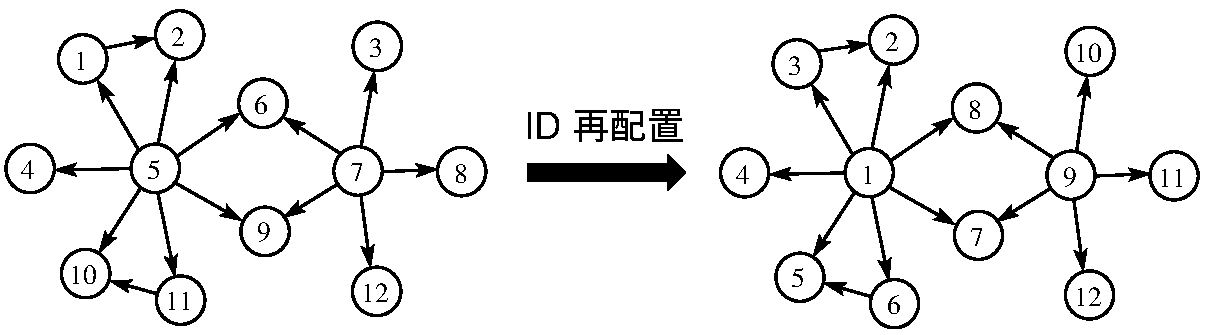
\includegraphics[width=\linewidth]{./figure/reordering_intro.pdf}
  \caption{ノード ID 再配置の例}
  \label{reordering_intro}
\end{figure}
RW で収集したグラフに対しても Reordering は有効であるが,既存の Reordering 手法は対象グラフの
全体構造が把握可能という制約条件が設定されている.
つまり,自律分散グラフ管理環境で既存の Reordering 手法を適用する場合,RW によるグラフ収集が完了するまで Reordering を実行できない.
Reordering を実行するまで収集したグラフはメモリ上で格納し続ける必要があるため,
収集するグラフサイズに比例したメモリ使用が発生してしまう.
\begin{comment}
  並列化による処理時間の減少についての評価も取るのであれば,ここで述べる
\end{comment}
人気コンテンツの周辺グラフなど収集したいグラフサイズが巨大な場合を想定すると,
自律分散グラフ管理環境におけるメモリ使用を抑えた Reorderin 手法が必要となる.

本研究では,自律分散グラフ管理環境においてメモリ使用を抑えるために,RW によるグラフ収集の途中で
部分的に Reordering を実行する手法として Sequential と Dynamic Degree Based Grouping (DDBG) を提案する.
そして,自律分散グラフ管理環境において Sequential, DDBG をそれぞれ実行した時の演算速度向上率,Reordering に伴うメモリ使用量
を明らかにする.
\section{本研究の位置付け}
TO DO

4分割のマトリックス的なやつを示し,SequentialとDBG-EEの立ち位置を,再配置に伴う特徴から明示する.
なぜか画像が表示されないんだがあ

\section{本論文の構成}
第1章では自律分散グラフ管理環境の概要と既存の Graph Reordering 手法の問題点を明示し,自律分散グラフ管理環境を想定した
Graph Reordering 手法の必要性を述べた.第2章では Graph Reordering の技術的な特徴を整理し,Reordering と グラフ演算時のキャッシュミス減少との
関係性について述べる.第3章では本論文の関連研究について述べる.第4章では提案手法である Sequential と DDBG について述べる.第5章では提案手法の
評価を行う.最後に第6章では本論文における結論と今後の課題について述べる.